\clearpage
\chapter{Reconstruction}
\section{2D Case} 
\label{sec:2Dcase}
\subsection{Polar Fourier Transform}
As mentioned in the previous section, several experiments produce diffraction patterns along azimuthal axis. There is only one unknown orientation angle in the collection of diffraction patterns. The independent orientation is rotation with respect to azimuth axis. 

The algorithm explained below will mainly focus on how to get general 2D projected structure from \Bmq. The construction of \Imq from \Bmq leave phases, which is nonunique \cite{saldin2010PhysB}. The information about the phases can be gotten by constraining the structure and the intensities as real-positive quantities. That information provides additional information from \Bmq to \Imq.

Phasing is an algorithm to find the structure from the missing phases of intensities. The way it works is by constraining any information about structure. The condition of electron density must be positive and real is imposed. In addition to that, several algorithms impose structure to be localized. Phasing is one of established algorithm that works by constraining prior information throughout iteration. A Similar method can be applied to impose a real space constraint iteratively in order to get structure from \Bmq.  

By definition, \Bmq is described in polar coordinate \cite{saldinNJournal}. To avoid interpolation, polar coordinate is chosen as a basis coordinate for real space and reciprocal space. The consequence of that it excludes FFT algorithm to be used inside iteration because FFT is defined in cartesian coordinate. The calculation of polar fourier transform is required and need to be formulated to go back and forth from real and reciprocal space. 

Any function can be decomposed into its basis function component. It is sensible to decompose function into its exponential components because the problem is related to the rotation of azimuthal angle. The decomposition of the electron density of the molecule is defined by
\begin{eqnarray}
\label{eq:rhorm}
\rho(r,\theta)=\sum_{m} \rho_{m}(r) \exp(i m \theta)
\end{eqnarray}
where $r$ and $\theta$ refer to a coordinate that can be sampled at polar point without interpolation. $\rho_{m}$ contain only radial dependence and the angular dependence is contained in $m$ components. 

Intensity is absolute square of Fourier transform of the electron density. The established FFT routines cannot be used owing to the fact that $\rho$ are sampled at polar coordinate. It is necessary to obtain a direct relation from electron density to intensity directly in polar coordinate. Fourier transform of $\rho(r,\theta)$ is shown below:
\begin{eqnarray}
\label{Aqpolarfourier}
A(\vec{q}) = \int d^{2}r \rho(r,\theta) \exp(i \vec{q} \cdot \vec{r}).  
\end{eqnarray}

In general, the structure factor is a fourier transform of electron density. As stated in equation \ref{Aqpolarfourier}, the structure factor is obtained by integrating over all electron density multiplied by a phase factor. All point are sampled in polar coordinates for both the electron density $(r,\theta)$ and the structure factor $(q,\theta_{q})$. 

One can relate exponential functions to Bessel function. The relation is called Jacobi Anger relation, which express exponential function into a sum of Bessel functions \cite{jacobianger}. The relation is
\begin{eqnarray}
\label{jacobanger}
\exp(i \vec{q} \cdot \vec{r} ) &=& \exp(i q r \cos( \theta_{q}-\theta_{r} ))  \\
&=& \sum_{m} i^{m} J_{m}(q r) \exp(i m ( \theta_{q}-\theta_{r} ) ). 
\end{eqnarray}
By substituting the Jacobi-Anger expansion into the Fourier transform of the electron density, a relation between structure factor, electron density and Bessel function is obtained: 
\begin{eqnarray}
\label{Amderive}
A(\vec{q}) &=& \int d^{2}r \rho(r,\theta) \exp(i \vec{q} \cdot \vec{r})  \\ 
&=& \int d^{2}r \sum_{m} \rho(r,\theta) i^m J_{m}(q r) \exp(i m ( \theta_{q}-\theta_{r} )).
\end{eqnarray}

\Bmq can be expressed in terms of an exponential decomposition of the intensity. By substituting equation \ref{rhom} into equation \ref{Amderive}, the structure factor can be expressed in terms of exponential decomposition. The derivation is shown below:
\begin{eqnarray}
\label{Amderive2}
A(\vec{q})&=& \int d^{2}r \sum_{m} \bigg[\sum_{m'} \rho_{m'}(r) \exp(i m' \theta_{r}) \bigg] i^m J_{m}(q r) \exp(i m ( \theta_{q}-\theta_{r} )) \\
&=& \int r dr \sum_{m',m} \rho_{m'}(r) i^m J_{m}(q r) \exp(i m ( \theta_{q})) \int d\theta_{r} \exp(i (m'-m) \theta_{r}).
\end{eqnarray}

Equation \ref{Amderive2} involve infinite integral of the exponential function. That integral is equivalent to the delta function \cite{deltafunction}, hence equation \ref{Amderive2} can be simplified become
\begin{eqnarray}
\label{deltafun}
\delta(m'-m)=\frac{1}{2 \pi} \int_{\infty}^{-\infty} \exp(i x(m'-m)) dx .
\end{eqnarray}
Thus, equation \ref{Amderive} can be written as
\begin{eqnarray}
\label{Amderive3}
A(\vec{q}) = \int r dr \sum_{m} \rho_m(r) i^m J_{m}(q r) 2 \pi \exp(i m ( \theta_{q})) . 
\end{eqnarray}
By decomposing left hand side of equation \ref{Amderive3} and equating each component in exponential term, a new relation is found that is 
\begin{eqnarray}
\sum_{m} A_{m}(q) \exp(i m \theta_{q}) = \sum_{m} \bigg[ 2 \pi \int r dr \rho_{m}(r) i^{m} J_{m}(q r) \bigg] \exp(i m \theta_{q}).  
\end{eqnarray}
The important relation between the structure factor decomposition and its exponential components can be obtained:
\begin{eqnarray}
\label{Am}
A_{m}(q) &=& 2 \pi \int rdr  \rho_{m}(r) i^m J_{m}(q r) .
\end{eqnarray}

In a similar way as the Fourier transform, the inverse Fourier transform is obtained by swaping $i$ to $-i$. It is generally accepted that electron density is the inverse Fourier transform of the structure factor. By using equation \ref{jacobanger} and equation \ref{deltafun}, the derivation is performed in the same way as polar Fourier transform. The following is the derivation:
\begin{eqnarray*}
\rho(\vec{r}) &=& \int d^{2}r A(q,\theta_{q}) \exp(-i \vec{q} \cdot \vec{r})  \\
&=& \int d^{2}q \sum_{m} A(q,\theta_{q}) (-i)^m J_{m}(q r) \exp(-i m ( \theta_{q}-\theta_{r} )) \\
&=& \int d^{2}q \sum_{m} \bigg[\sum_{m'} A_{m'}(q) \exp(i m' \theta_{q}) \bigg] (-i)^m J_{m}(q r) \exp(-i m ( \theta_{q}-\theta_{r} )) \\
&=& \int q dq \sum_{m',m} A_{m'}(q) (-i)^m J_{m}(q r) \exp(i m ( \theta_{r})) \int d\theta_{q} \exp(i (m'-m) \theta_{q}) \\
&=& \int q dq \sum_{m} A_m(q) (-i)^m J_{m}(q r) \exp(i m ( \theta_{r})) 2 \pi \\
\sum_{m} \rho_{m}(r) \exp(i m \theta_{r}) &=& \sum_{m} \bigg[ 2 \pi \int q dq A_{m}(q) (-i)^{m} J_{m}(q r) \bigg] \exp(i m \theta_{r}). 
\end{eqnarray*}
Because now the left hand side and the previous right hand side of the equation have the exponential terms, equating each component will lead to a new important equation. The relation between the exponential components of the electron density and the exponential component of the structure factor can be obtained: 
\begin{eqnarray}
\label{rhom}
\rho_{m}(r) &=& 2 \pi \int qdq  A_{m}(q) (-i)^m J_{m}(q r).
\end{eqnarray}

Equations \ref{Am} and \ref{rhom} are the foundation to do Fourier transform in polar coordinates directly without involving the cartesian space. After obtaining the exponential components of the structure factor or the electron density, the summation with respect to its basis function is performed to get $\rho(\vec{r})$ or $A(\vec{q})$ as shown
\begin{eqnarray}
\label{rho_aq}
\rho(\vec{r})&=&\sum_{m} \rho_{m}(r) \exp(i m \theta)  \\
A(\vec{q})&=&\sum_{m} A_{m}(q) \exp(i m \theta). \nonumber 
\end{eqnarray}

\subsection{Angular Correlation Constraint}
As explained earlier, the correlation methods need to calculate \Bmq from experiment. Information of intensity should be obtained from \Bmq and the other constraints. Phasing algorithm can be modified so that the constraint is on \Bmq instead of intensity\cite{Donatelli}. The step is explained as follow:
\begin{figure}[ht]
  \centering
  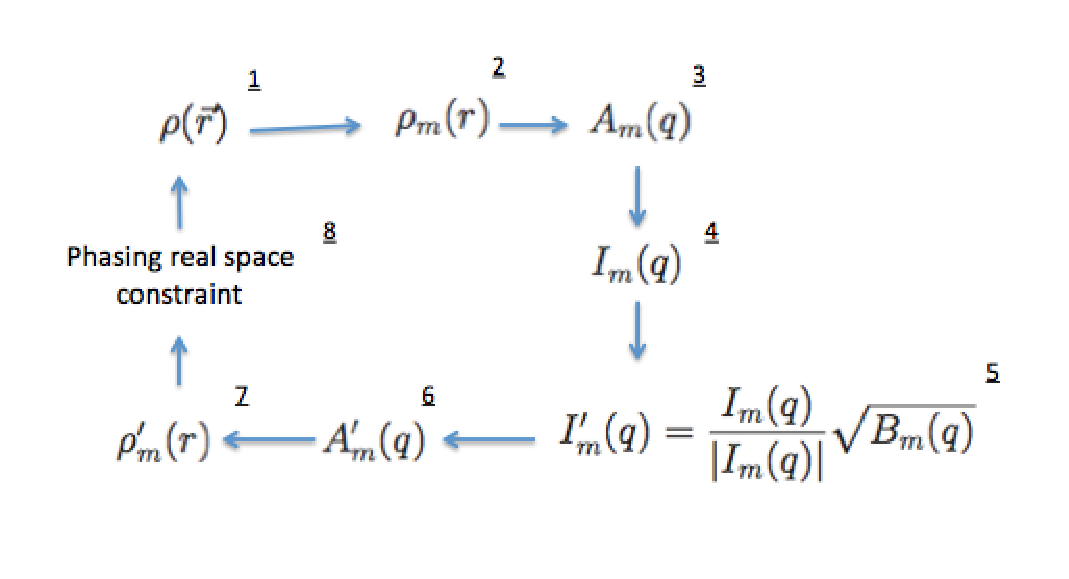
\includegraphics[width=.8\textwidth]{Bconstraint}
\caption{Full cycle of phasing algorithm with $B_{m}(q,q)$ as constraint}
\label{fig:Bconstraint}
\end{figure}
\begin{enumerate}
  \item Start initial guess of $\rho(\vec{r})$
  \item Calculate $\rho_{m}(q)$ from $\rho(\vec{r})$
  \item Use equation \ref{Am} to calculate $A_{m}(q)$
  \item Calculate $I_{m}(q)$ from $A_{m}(q)$ and keep information of phase. \\
    Start from calculating $A(\vec{q})=\sum_{m} A_{m}(\vec{q}) \exp(i m \theta)$ then $I(\vec{q})=|A(\vec{q})|^{2}$. \\
    Final step is $I_{m}(q)=\int I(\vec{q}) \exp(-i m \theta) d\theta $ 
  \item Project $I_{m}(q)$ to satisfy $B_{m}(q,q)$ constraint
  \item Use phase from step 4 to obtain $A'_{m}(q)$ 
  \item Calculate $\rho_{m}(q)$ from equation \ref{rhom}
  \item Use HIO, ER, and shrinkwrap to constraint $\rho(\vec{r})$ and cycle is repeated
\end{enumerate}
\begin{figure}[ht]
  \centering
  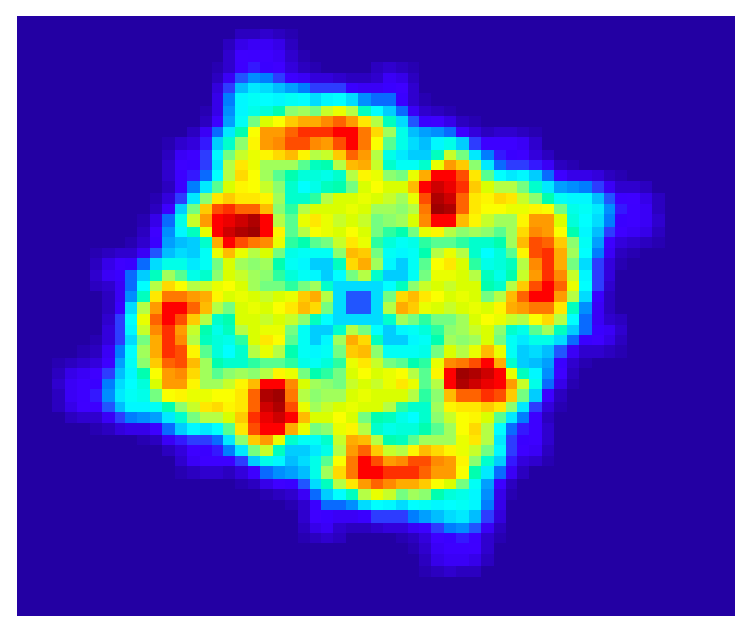
\includegraphics[width=.3\textwidth]{kc2dmodel}
\caption{ Electron density of K channel protein is used as a model to calculate $B_{m}(q,q)$}
\label{fig:kc2dmodel}
\end{figure}
\begin{figure}[ht]
  \centering
  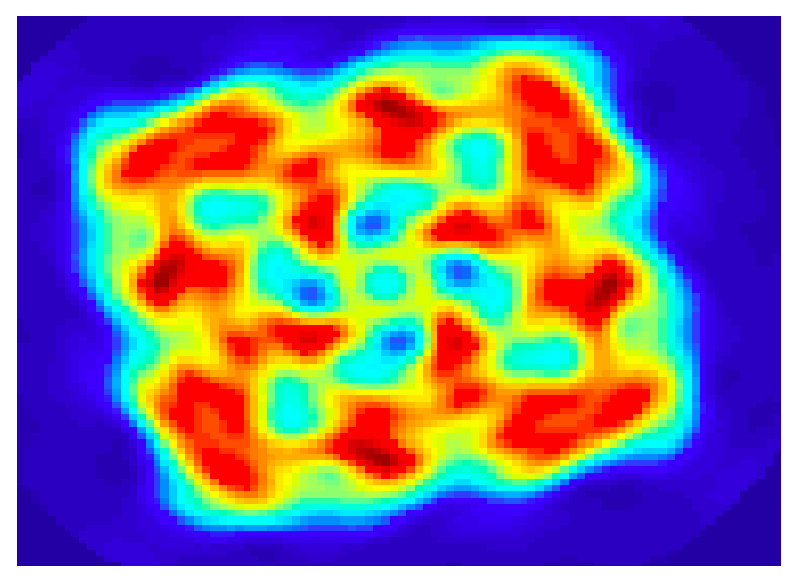
\includegraphics[width=.27\textwidth]{kc2drec}
\caption{Reconstruction of electron density by only constraining to diagonal value of $B_{m}(q,q)$}
\label{fig:kc2drec}
\end{figure}
Figure \ref{fig:kc2dmodel} is model that is used simulate $B_{m}(q,q)$. 
After applying phasing constraint on $B_{m}(q,q)$, the reconstruction is shown on figure \ref{fig:kc2drec}. 

Important to note that in this reconstruction only information on diagonal value of $B_{m}(q,q)$ is used.  
Another important quantity is R-factor, R-factor between \Bmq model and its reconstruction is $0.15$, which is defined as
\begin{eqnarray}
R_{factor}=\frac{\sum ||B_{m}(q,q)|-|B_{m}(q,q)_{exp}||}{\sum |B_{m}(q,q)_{exp}|}. 
\end{eqnarray}
Judging from figure \ref{fig:kc2drec} and R-factor, the reconstruction is reasonable enough even though only diagonal values are used as constraint. The discrepancy between model and reconstruction could be attributed to the fact that only diagonal values of $B_{m}(q,q)$ are used. 


